\documentclass[crop,tikz]{standalone}% 'crop' is the default for v1.0, before it was 'preview'
%\usetikzlibrary{...}% tikz package already loaded by 'tikz' option
\usepackage{color}
\newcommand{\gv}[1]{\ensuremath{\mbox{\boldmath$ #1 $}}} 
\renewcommand{\v}[1]{\ensuremath{\mathbf{#1}}}
\newcommand{\name}[1]{_{\text{#1}}}
\usepackage{siunitx}
\usetikzlibrary{shapes,arrows,shadings,backgrounds,calc}
\definecolor{brown}{rgb}{0.59, 0.29, 0.0}
\begin{document}
\fontfamily{cmss}
{\begin{tikzpicture}

  \node[label={[xshift=-2.1cm,yshift=-1.25cm]\Large A}](a) at (0,0) {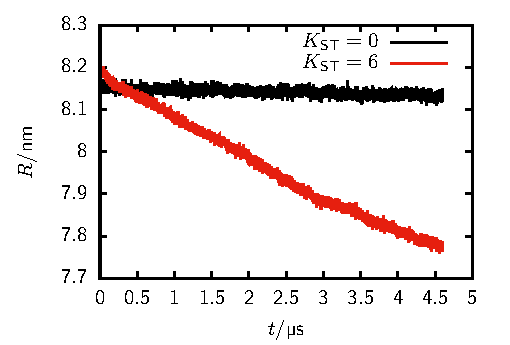
\includegraphics{radius.pdf}};
  \begin{pgfonlayer}{background}

    \node at ([xshift=-0.250cm,yshift=-0.5cm]a) (c) {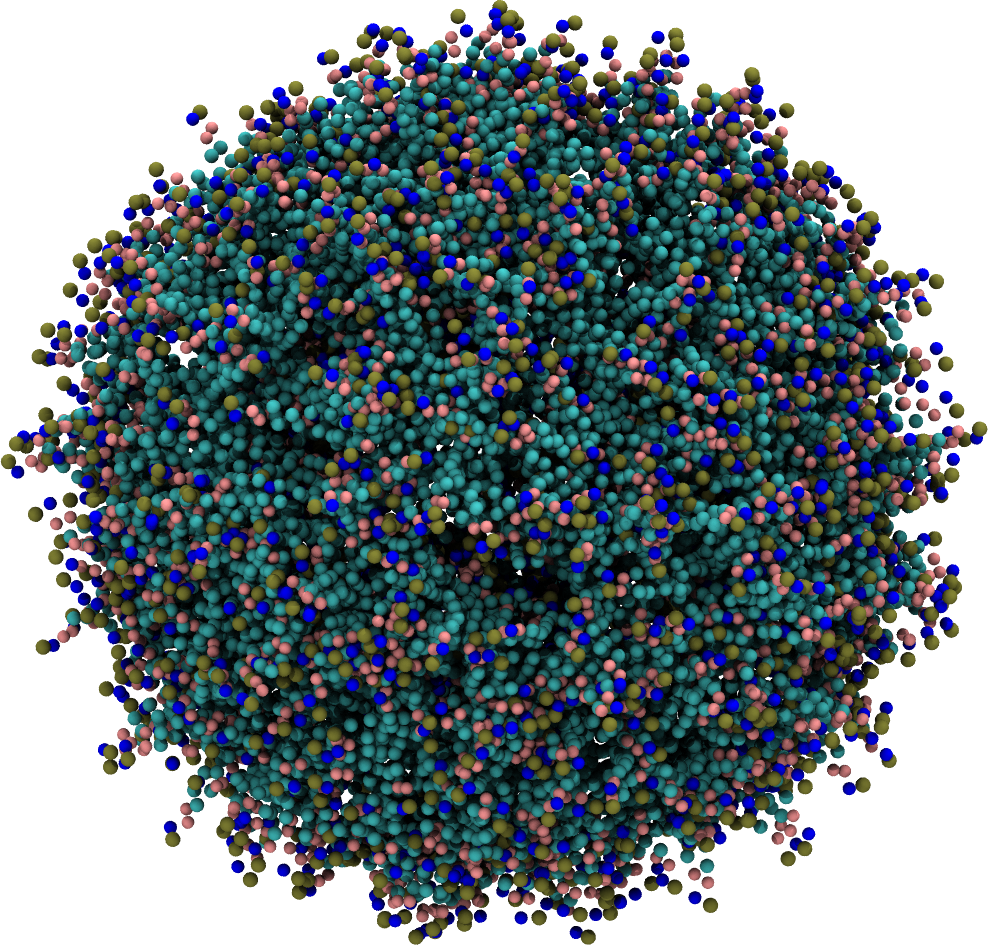
\includegraphics[width=0.75in]{start.png}};

%    \node at ([xshift=0.5cm,yshift=-0.5cm]a) (c) {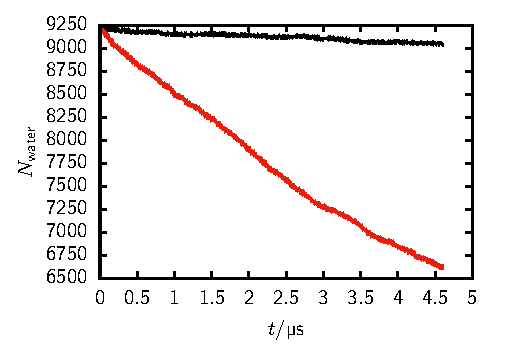
\includegraphics{water_inside.pdf}};

    \draw[->,ultra thick](-2.6cm,-1.3cm)--node[above,sloped] {initial}(c);
  \end{pgfonlayer}
  \node[label={[xshift=-2.1cm,yshift=-1.25cm] \Large B},fill=white](b) at (0,-5) {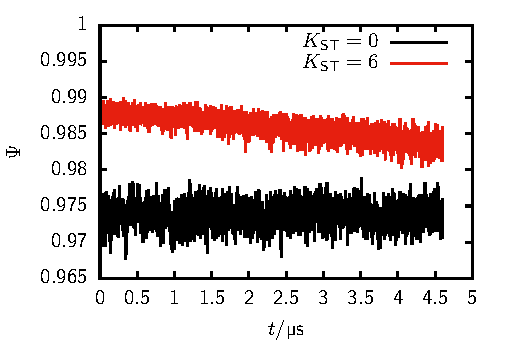
\includegraphics{sphericity.pdf}};

  \node[label={[xshift=-2.1cm,yshift=-1.25cm,fill=white,opacity=0.8,text opacity=1]\Large C},right of=a,node distance=8cm] (c) {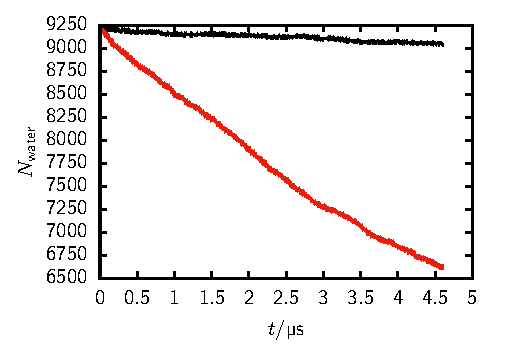
\includegraphics{water_inside.pdf}};

  
  \node[right of=b,node distance=6cm,label=above:{\Large $K_{\text{ST}}=0$},yshift=-1cm]  (e) {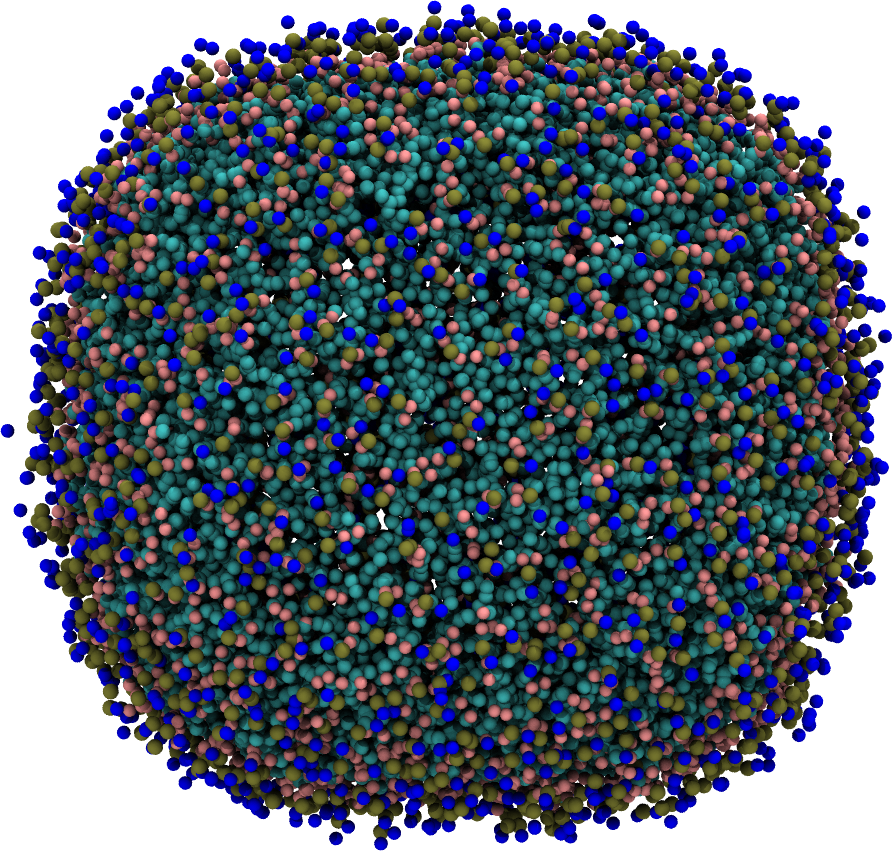
\includegraphics[width=1.5in]{vesicle_0.png}};


  
  \node[right of=e,node distance=4.5cm,label=above:{\Large $K_{\text{ST}}=6$}]  (g) {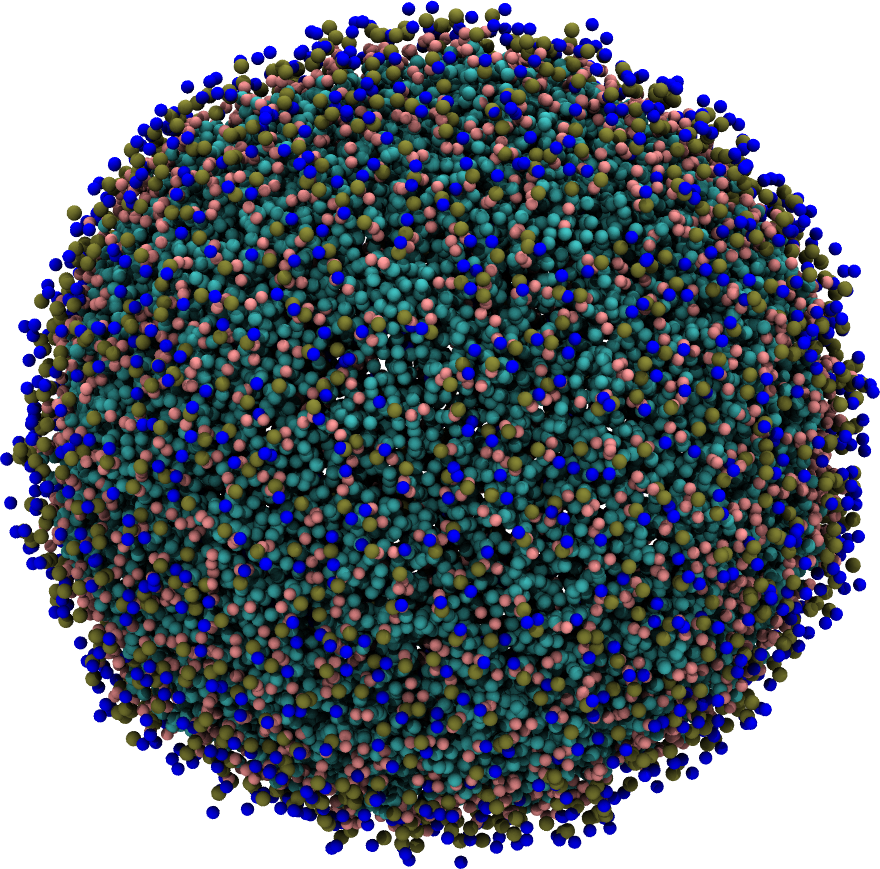
\includegraphics[width=1.5in]{vesicle_6.png}};

  

  
\end{tikzpicture}
}
\end{document}
